%\chapter{Desarrollo de aplicaciones ADAS basadas en CV y medio de pruebas de control}
\chapter{Casos de estudio bajo funcionamiento exacto}
\label{ch:visioncontrol}

\section{Aplicaciones seleccionadas}

Las selección de las ADAS se hizo luego de realizar la taxonomía. Esto debido a que luego de esa etapa se tenían las bases para escoger. Ante la cantidad de ADAS recopiladas se precisó de un medio de selección para determinar cuales se iban a utilizar para la exploración. Esta selección se basó en 3 puntos:
\begin{itemize}
    \item Disponibilidad inmediata del sensor
    
        Siendo 3 disponible y 0 no disponible
    
    \item Criticidad de no funcionamiento
    
        Siendo 3 muy crítico y 0 nada crítico  
    
    \item Facilidad de implementación
    
        Siendo 3 fácil de implementar y 0 complejo de implementar
\end{itemize}

Se creó una la Tabla 3.1 donde se muestran los valores de cada ADAS según el rubro a evaluar en cada columna y se obtuvo resultados, sumando los valores, en los que particularmente 4 ADAS sobresalieron: TSR, PPS, DSM y LDW. De estas se obtuvo finalmente una lista de las 3. Para simplificarlo se escogieron TSR, PPS y LDW debido a que, de acuerdo a los niveles de autonomía, proporcionan información relevante al vehículo en lo que concierne a su desplazamiento. La DSM si bien es importante debido a su alerta de fatiga no aporta más allá que eso.


\begin{table}[H]
\centering
\caption{Valores para selección}
\label{my-label}
\begin{tabular}{|c|c|c|c|c|}
\hline
ADAS & \begin{tabular}[c]{@{}l@{}}Disponibilidad de \\ sensor utilizado\end{tabular} & \begin{tabular}[c]{@{}l@{}}Criticidad de\\ no funcionamiento\end{tabular} & Implementación & Total \\\hline
TCS  & 2                                                                             & 3                                                                         & 1              & 6     \\
ESC  & 2                                                                             & 3                                                                         & 1              & 6     \\
ACC  & 3                                                                             & 1                                                                         & 2              & 6     \\
ISA  & 1                                                                             & 1                                                                         & 2              & 4     \\
TSR  & 3                                                                             & 3                                                                         & 2              & 8     \\
SLR  & 3                                                                             & 2                                                                         & 2              & 7     \\
AEB  & 2                                                                             & 3                                                                         & 2              & 7     \\
PPS  & 3                                                                             & 3                                                                         & 2              & 8     \\
PCW  & 2                                                                             & 3                                                                         & 1              & 6     \\
CAS  & 2                                                                             & 3                                                                         & 1              & 6     \\
NS   & 2                                                                             & 1                                                                         & 2              & 5     \\
DSM  & 3                                                                             & 3                                                                         & 2              & 8     \\
BSD  & 1                                                                             & 3                                                                         & 2              & 6     \\
LDW  & 3                                                                             & 3                                                                         & 2              & 8     \\
LCA  & 3                                                                             & 2                                                                         & 2              & 7     \\
RVC  & 3                                                                             & 1                                                                         & 3              & 7     \\
IPA  & 2                                                                             & 1                                                                         & 2              & 5     \\
NV   & 1                                                                             & 2                                                                         & 2              & 5     \\
AFS  & 2                                                                             & 2                                                                         & 2              & 6     \\
RSS  & 2                                                                             & 1                                                                         & 3              & 6  \\\hline  
\end{tabular}
\end{table}

Las 3 aplicaciones escogidas son claves para alcanzar ese ansiado nivel 5 de autonomía en la conducción de vehículos.


\subsection{Alerta de Salida del Carril (LDW)}

La detección de carril es fundamental si se desea llegar a ese nivel 5 de autonomía, esto le daría al usuario la tranquilidad de que el vehículo en el que se encuentre va a ser capaz de mantenerse en su carril y no invadir otros, de esta manera accidentes por invasión de carril tanto en el mismo sentido como en sentido contrario de conducción se erradicarían haciendo las calles más seguras.
\newpage
\subsection{Control de Alerta de Peatones (PPS)}

Los peatones si bien no son usuarios propios de las carreteras, pueden estar presentes en ellas. Ya sea por necesidad de cruzar, por que caminan por el espaldón, por la razón que sea no se puede descartar su presencia en las carreteras. Lo que sí se puede hacer es tomar medidas ante la posible aparición de estos en las vías, de esta manera la meta es reducir las estadísticas de atropellos a peatones. 

\subsection{Reconocimiento de Se~nales de Transito (TSR)}

Las señales de transito son indispensables para que el conductor tenga las instrucciones necesarias y delimitar el accionar de estos en las carreteras. Velocidades permitidas, avisos, restricciones, indicaciones de lugares, etc. En este caso nos vamos a enfocar en señales de velocidades permitidas, de este modo indicarle al sistema en que valores de velocidad debe mantenerse según las señalización vertical de las carreteras.

\section{Descripción del capítulo}

El primer caso de estudio comprende en observar el funcionamiento exacto de aplicaciones ADAS, es decir, trabajando tal y como se plantea en los artículos científicos leídos. Se procede a poner en marcha las 3 aplicaciones seleccionadas (TSR, LDW y PCW), todas basadas en CV, para luego probarlas en un sistema de control y obtener una referencia ante que comparar lo que se va a explorar en el siguiente caso de estudio que se presenta en el capítulo 4. Se introducen entonces, los conceptos necesarios para el adecuado entendimiento de lo que este capitulo consiste. 


\subsection*{Visión por Computadora}

La Visión por Computadora (CV), también llamada Visión Artificial, es la transformación de datos de una cámara fotográfica fija o de video en una decisión o una nueva representación. Todas estas transformaciones se hacen para lograr algún objetivo en particular. Los datos de entrada pueden incluir alguna información contextual como "la cámara está montada en un vehículo" o "el láser indica que un objeto está a 1 metro de distancia". La decisión podría ser "hay una persona en esta escena" o "hay 14 células tumorales en esta diapositiva". Una nueva representación puede significar convertir una imagen de color en una imagen en escala de grises o quitar el movimiento de la cámara de una secuencia de imágenes.\cite{Bradski2008}

A pesar de que somos criaturas visuales, es fácil ser engañado en pensar que las tareas de la visión de computadora son fáciles. ¿Qué tan difícil puede ser encontrar un coche cuando lo miras fijamente en una imagen? Sus intuiciones iniciales pueden ser bastante engañosas. El cerebro humano divide la señal de la visión en muchos canales que fluyen diferentes tipos de información en su cerebro. El cerebro tiene un sistema de atención que identifica, de manera dependiente de la tarea, partes importantes de una imagen para examinar mientras se reprime el examen de otras áreas. Hay retroalimentación masiva en el flujo visual que es, hasta ahora, poco entendido. Existen insumos asociativos generalizados de los sensores de control muscular y de todos los otros sentidos que permiten al cerebro dibujar en asociaciones cruzadas hechas a partir de años de vida en el mundo. Los bucles de retroalimentación en el cerebro se remontan a todas las etapas de procesamiento, incluyendo los propios sensores de hardware (los ojos), que controlan mecánicamente la iluminación a través del iris y afinan la recepción en la superficie de la retina. La visión de la computadora es un campo que crece rápidamente, en parte como resultado de cámaras más baratas y más capaces, en parte debido a la energía de proceso comprable, y en parte porque los algoritmos de la visión están comenzando a madurar. OpenCV en sí ha desempeñado un papel en el crecimiento de la visión de la computadora al permitir que miles de personas hagan un trabajo más productivo en la visión. Con su enfoque en la visión en tiempo real, OpenCV ayuda a los estudiantes y profesionales a implementar eficientemente proyectos y a iniciar la investigación, proporcionándoles una visión de la computadora y la infraestructura de aprendizaje de máquinas que anteriormente estaba disponible sólo en unos pocos laboratorios de investigación madura.\cite{Bradski2008}

\subsection*{Control Automático}

En esta sección se pretende dar una visión general de lo que el Control Automático significa y para ello se comienza con una serie de conceptos básicos recopilados de \cite{Ogata2013} los cuales se exponen a continuación:

La \textbf{variable controlada} es la cantidad o condición que se mide y controla. 
La \textbf{señal de control} es la cantidad o condición que el controlador modifica para afectar el valor de la variable controlada.

\textbf{Controlar} significa medir el valor de la variable controlada del sistema y aplicar la variable manipulada al sistema para corregir o limitar la desviación del valor medido respecto del valor deseado. En el estudio de la ingeniería de control, es necesario definir términos adicionales que se precisan para describir los sistemas de control.

Una \textbf{planta} puede ser una parte de un equipo, tal vez un conjunto de los elementos de una máquina que funcionan juntos, y cuyo objetivo es efectuar una operación particular. En este libro se llamará planta a cualquier objeto físico que se va a controlar (como un dispositivo mecánico, un horno de calefacción, un reactor químico o una nave espacial).

El Diccionario Merriam-Webster define un \textbf{proceso} como una operación o un
desarrollo natural progresivamente continuo, marcado por una serie de cambios graduales que se suceden unos a otros de una forma relativamente fija y que conducen a un resultado o propósito determinados; o una operación artificial o voluntaria que se hace de forma progresiva y que consta de una serie de acciones o movimientos controlados, sistemáticamente dirigidos hacia un resultado o propósito determinado. En este libro se llamará proceso a cualquier operación que se va a controlar. Algunos ejemplos son los procesos químicos, económicos y biológicos.

Un \textbf{sistema} es una combinación de componentes que actúan juntos y realizan un objetivo determinado. Un sistema no está necesariamente limitado a los sistemas físicos. El concepto de sistema se puede aplicar a fenómenos abstractos y dinámicos, como los que se encuentran en la economía. Por tanto, la palabra sistema debe interpretarse en un sentido amplio que comprenda sistemas físicos, biológicos, económicos y similares.

Una \textbf{perturbación}  es una señal que tiende a afectar negativamente el valor de la salida de un sistema. Si la perturbación se genera dentro del sistema se denomina interna, mientras que una perturbación externa se genera fuera del sistema y es una entrada.

El \textbf{control realimentado} se refiere a una operación que, en presencia de perturbaciones, tiende a reducir la diferencia entre la salida de un sistema y alguna entrada de referencia, y lo realiza tomando en cuenta esta diferencia. Aquí sólo se especifican con este término las perturbaciones impredecibles, ya que las perturbaciones predecibles o conocidas siempre pueden compensarse dentro del sistema

\subsection*{Tipos de Controladores}
\subsubsection*{Lazo Cerrado vs Lazo Abierto}

Sistemas de control en lazo cerrado en comparación con sistemas en lazo abierto. Una ventaja del sistema de control en lazo cerrado es que el uso de la realimentación vuelve la respuesta del sistema relativamente insensible a las perturbaciones externas y a las variaciones internas en los parámetros del sistema. Es así posible usar componentes relativamente poco precisos y baratos para obtener el control adecuado de una planta determinada, mientras que hacer eso es imposible en el caso de un sistema en lazo abierto. Desde el punto de vista de estabilidad, el sistema de control en lazo abierto es más fácil de desarrollar, porque la estabilidad del sistema no es un problema importante. Por otra parte, la estabilidad es un gran problema en el sistema de control en lazo cerrado, que puede conducir a corregir en exceso errores que producen oscilaciones de amplitud constante o cambiante. Debe señalarse que, para los sistemas en los que se conocen con anticipación las entradas y en los cuales no hay perturbaciones, es aconsejable emplear un control en lazo abierto. Los sistemas de control en lazo cerrado sólo tienen ventajas cuando se presentan perturbaciones y/o variaciones impredecibles en los componentes del sistema. El número de componentes usados en un sistema de control en lazo cerrado es mayor que el que se emplea para un sistema de control equivalente en lazo abierto. Por tanto, el sistema de control en lazo cerrado suele tener costes y potencias más grandes. Para disminuir la potencia requerida de sistema, se emplea un control en lazo abierto siempre que pueda aplicarse. Por lo general, una combinación adecuada de controles en lazo abierto y en lazo cerrado es menos costosa y ofrecerá un comportamiento satisfactorio del sistema global.
En ciertas circunstancias (por ejemplo, si no hay perturbaciones o la salida es difícil de medir) pueden ser deseables los sistemas de control en lazo abierto. Por tanto, es conveniente resumir las ventajas y desventajas de utilizar sistemas de control en lazo abierto\cite{Ogata2013}

\subsubsection*{Controlador P }

La acción de control proporcional, da una salida del controlador que es proporcional al error y puede
controlar cualquier planta estable, pero posee desempeño limitado y error en régimen permanente\cite{Mazzone2012}.

\subsubsection*{Controlador I }

Da una salida del controlador que es proporcional al error acumulado, lo que implica que es un modo de controlar lento\cite{Mazzone2012}.

\subsubsection*{Controlador PI }

Con un control proporcional, es necesario que exista error para tener una acción de control distinta de cero. Con acción integral, un error pequeño positivo siempre nos dará una acción de control creciente, y si fuera negativo la señal de control ser a decreciente. Este razonamiento sencillo nos muestra que el error en régimen permanente sera siempre cero. Muchos controladores industriales tienen solo acción PI. Se puede demostrar que un control PI es adecuado para todos los procesos donde la dinámica es esencialmente de primer orden\cite{Mazzone2012}.

\subsubsection*{Controlador PD }

Esta acción tiene carácter de previsión, lo que hace más rápida la acción de control, aunque tiene la desventaja importante que amplifica las señales de ruido y puede provocar saturación en el actuador. La acción de control derivativa nunca se utiliza por sí sola, debido a que solo es eficaz durante perıodos transitorios. Cuando una acción de control derivativa se agrega a un controlador proporcional, permite obtener un controlador de alta sensibilidad, es decir que responde a la velocidad del cambio del error y produce una corrección significativa antes de que la magnitud del error se vuelva demasiado grande.

\subsubsection*{Controlador PID }

Esta acción combinada reúne las ventajas de cada una de las tres acciones de control individuales\cite{Mazzone2012}.
\newpage


\section{Visión por Computadora}

Las aplicaciones ADAS seleccionadas, se desarrollan y adaptan para obtener resultados que, en una primera versión, son aceptables y muestran de manera general lo que se quiere realizar en cada una de ellas en su versión final. Mediante programación en c++ y las librerías y funciones específicas de OpenCV se logró obtener resultados provisionales del avance hasta el día de la presentación de este avance.


\subsection{Resultados para primer avance}
\subsubsection{LDW}

Lo obtenido al programar la LDW es lo que se presenta en la Figura 3.1. En la fila superior se muestra con lineas finas amarillas la Región de Interés (ROI) que es zona que se quiere estudiar, de esta manera solo procese esta y no la totalidad de la imagen, esto a manera de preprocesamiento. Seguidamente se genera una vista "Bird Eye" o vista de pájaro a partir de la ROI seleccionada anteriormente de este modo ya se cuenta con un panorama más claro y sencillo de estudiar. A este se le detectan bordes y se trazan lineas sobre ellos y se obtiene así la vista que se encuentra en la esquina superior derecha de la Figura 3.1. Finalmente se le realiza reacomoda en la imagen original se logra observar en la vista inferior de la Figura 3.1 que las indicaciones rojas calzan sobre las lineas. En dicha figura se muestra un cuadro del video completo, pero la aplicación corre sobre una grabación de un vehículo andando. Se puede observar un video de esta primera versión en: \url{https://youtu.be/myVD5Tk01nE}

\begin{figure}[H]
  \centering
  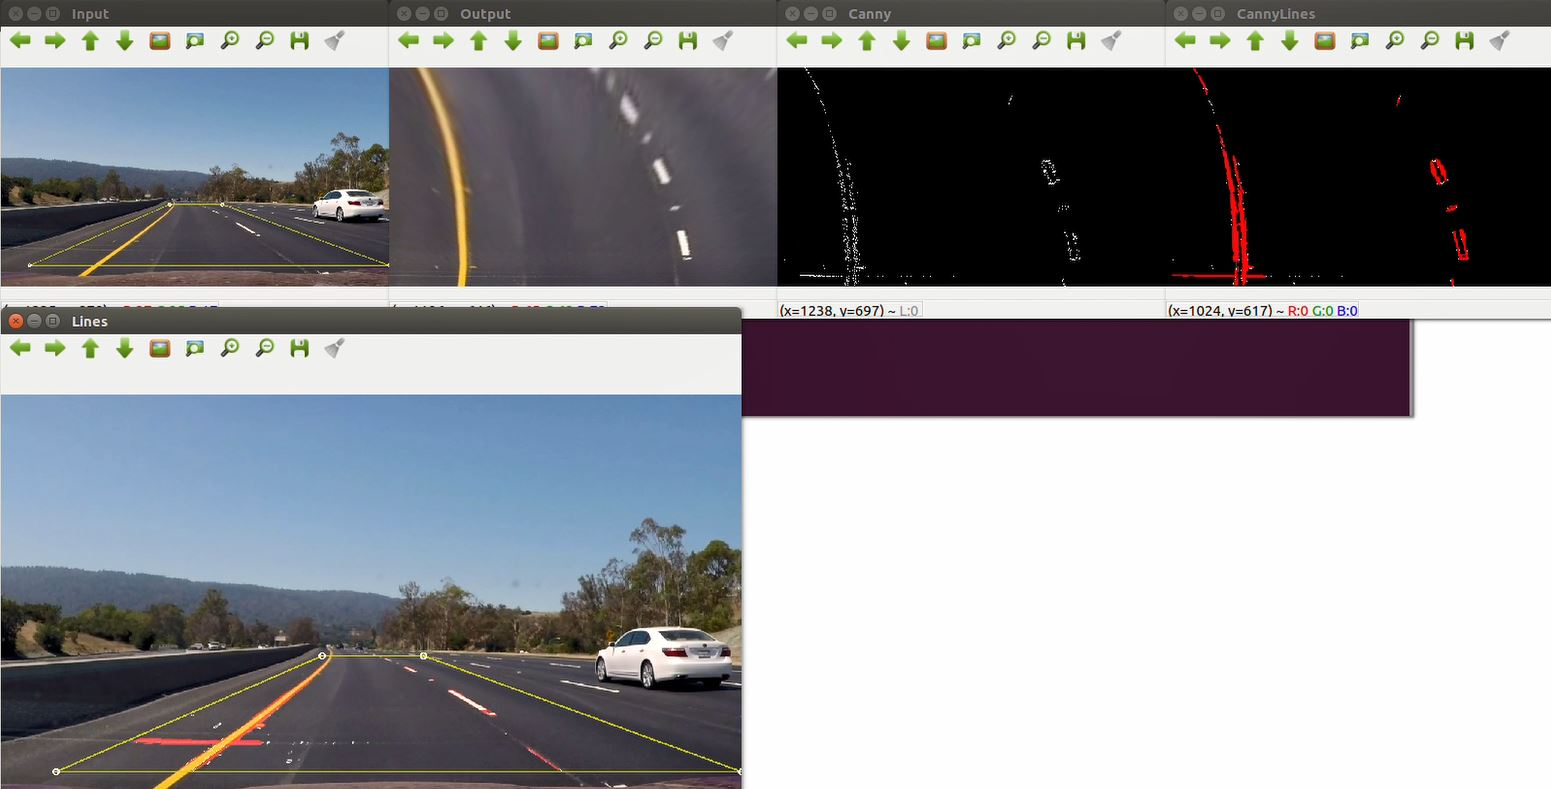
\includegraphics[width=0.9\textwidth]{ldw.JPG}
  \caption{Primeros resultados LDW}
  \label{fig:boat2}
\end{figure}


\begin{figure}[H]
  \centering
      \begin{tikzpicture}[node distance = 1.5cm, auto]
        % Place nodes
        \node [block] (init) {inicio};
        \node [block, below of=init] (prepro) {pre-procesamiento y demarcación de ROI};
        \node [block, below of=prepro] (detect) {detectar ROI};
        \node [block, below of=detect] (bird) {transformacion vista de pájaro};
        \node [block, below of=bird] (canny) {detectar bordes};
        \node [block, below of=canny] (lines) {trazar líneas};
        \node [decision, below of=lines] (decide) {¿Está centrado?};
        \node [block, below of=decide, node distance=3cm] (stop) {Emita alerta};
        \node [block, right of=canny, node distance=5cm] (update) {siguiente cuadro};
        % Draw edges
        \path [line] (init) -- (prepro);
        \path [line] (prepro) -- (detect);
        \path [line] (detect) -- (bird);
        \path [line] (bird) -- (canny);
        \path [line] (canny) -- (lines);
        \path [line] (lines) -- (decide);
        \path [line] (decide) -- node {si}(stop);
        \path [line,dashed] (stop) -| (update);
        \path [line] (decide) -| node [near start] {no}(update);
        \path [line,dashed] (update) |- (detect);
    \end{tikzpicture}    
  \caption{Diagrama flujo LDW propuesta}
  \label{fig:diag_ldw}
\end{figure}

\newpage


\subsubsection{PPS}

El detector de peatones se presenta en la Figura 3.2. En ella se observan 4 vistas de los pasos que se iban realizando para la obtención del resultado deseado. Los 2 cuadros del centro de la figura son pasos de preprocesamiento para finalmente poder aplicar una herramienta de detección de personas mediante cascada. Se puede observar un par de videos de esta primera versión en: \url{https://youtu.be/Rxt\_fKXrZTA} y en \url{https://youtu.be/pQZbL1H1IKk}

\begin{figure}[H]
  \centering
    \begin{tikzpicture}[node distance = 1.5cm, auto]
        % Place nodes
        \node [block] (init) {inicio};
        \node [block, below of=init] (prepro) {pre-procesamiento y demarcación de ROI};
        \node [block, below of=prepro] (roi1) {detectar peatón};
        \node [decision, below of=roi1] (decide) {¿Peatón en ROI?};
        \node [block, below of=decide, node distance=2.5cm] (stop) {Emita alerta};
        \node [block, right of=roi1, node distance=6cm] (update) {siguiente cuadro};
        % Draw edges
        \path [line] (init) -- (prepro);
        \path [line] (prepro) -- (detect);
        \path [line] (detect) -- (roi1);
        \path [line] (roi1) -- (decide);
        \path [line] (decide) -- node {si}(stop);
        \path [line,dashed] (stop) -| (update);
        \path [line] (decide) -| node [near start] {no}(update);
        \path [line,dashed] (update) -- (roi1);
    \end{tikzpicture}    
  \caption{Diagrama flujo PPS propuesta}
  \label{fig:diag_pps}
\end{figure}

\begin{figure}[H]
  \centering
  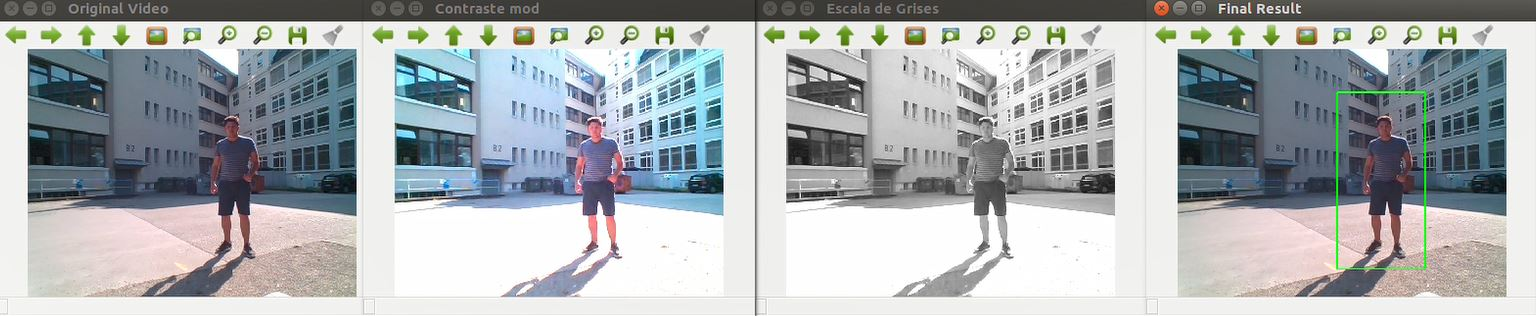
\includegraphics[width=0.8\textwidth]{pcw.JPG}
  \caption{Primeros resultados PPS }
  \label{fig:boat2}
\end{figure}
\newpage

\subsubsection{TSR}
El detector de señales de tránsito actualmente está en desarrollo. Del video fuente se detecta mediante cascada la zona que se desea analizar. Esta zona se asigna como ROI y se despliega en una ventana aparte. Al centro abajo de la Figura 3.3 se muestra una imagen que funciona como referencia ante que comparar la ROI seleccionada. Se pretende mediante comparación de histogramas determinar si la ROI es igual o compatible con la imagen de referencia. Para no meter ruido al histograma se debe generar otra ROI donde se elimine el anillo oscuro alrededor del número de la señal detectada. Se puede observar un de video de esta primera versión en: \url{https://youtu.be/Ku82Fxoz5P0}


\begin{figure}[H]
  \centering
    \begin{tikzpicture}[node distance = 1.5cm, auto]
        % Place nodes
        \node [block] (init) {inicio};
        \node [block, below of=init] (prepro) {pre-procesamiento};
        \node [block, below of=prepro] (detect) {detectar señal};
        \node [block, below of=detect] (roi1) {demarcar la señal como ROI};
        \node [block, below of=roi1] (roi2) {demarcar los dígitos con una ROI};
        \node [decision, below of=roi2] (decide) {¿Nuevo límite?};
        \node [block, below of=decide, node distance=2.25cm] (stop) {Despliegue valor de velocidad};
        \node [block, right of=roi2, node distance=5cm] (update) {siguiente cuadro};
        % Draw edges
        \path [line] (init) -- (prepro);
        \path [line] (prepro) -- (detect);
        \path [line] (detect) -- (roi1);
        \path [line] (roi1) -- (roi2);
        \path [line] (roi2) -- (decide);
        \path [line] (decide) -- node {si}(stop);
        \path [line,dashed] (stop) -| (update);
        \path [line] (decide) -| node [near start]{no}(update);
        \path [line,dashed] (update) |- (detect);
    \end{tikzpicture}    
  \caption{Diagrama flujo TRS propuesta}
  \label{fig:diag_tsr}
\end{figure}


\begin{figure}[H]
  \centering
  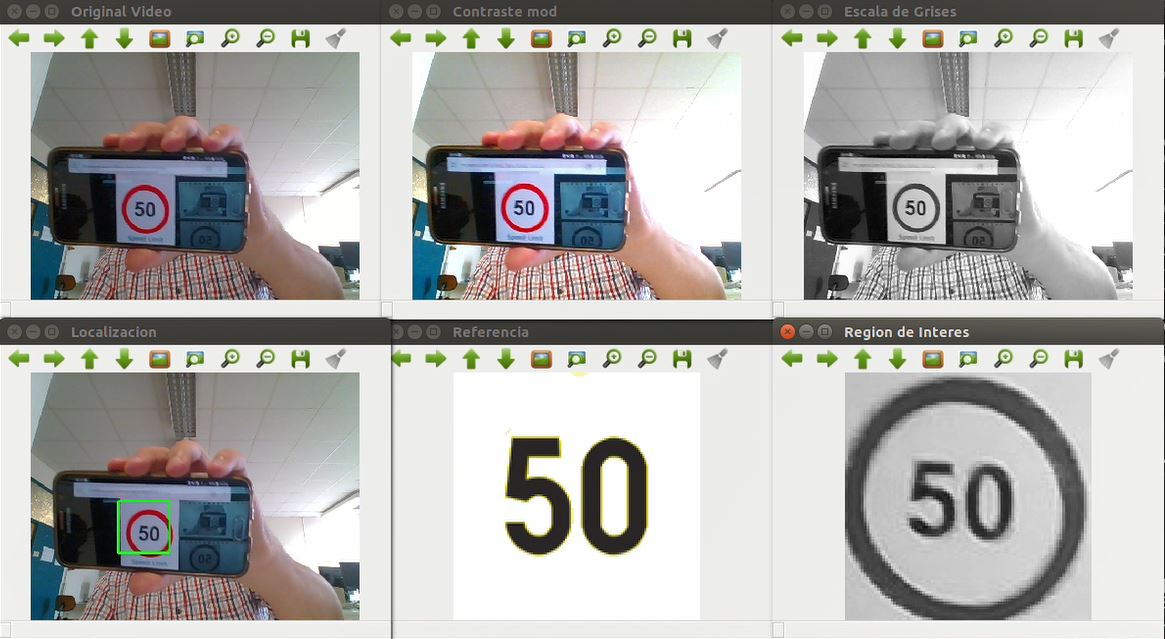
\includegraphics[width=0.45\textwidth]{tsr.JPG}
  \caption{Primeros resultados TSR}
  \label{fig:results_trs}
\end{figure}